\section{Affichage et visualisation des cours}
%http://www.simpleentrepreneur.com/2007/06/07/16-librairies-et-scripts-pour-generer-des-graphiques-sur-internet/
%http://www.fusioncharts.com/goodies/fusioncharts-free/
%http://docs.fusioncharts.com/free/#_ga=1.124638285.613042136.1459322699
%https://fr.wikipedia.org/wiki/Adobe_Flash
%http://www.tutorialspoint.com/jfreechart/jfreechart_overview.htm
%http://www.jfree.org/jfreechart/
%http://www.jfree.org/phpBB2/viewtopic.php?t=9621


L'un des objectifs de notre projet étant de fournir à l'utilisateur une IHM pour visualiser les cours ainsi que des indicateurs financiers via l'analyse technique que nous verrons dans le chapitre suivant, nous avons besoin d'afficher des graphes et autres diagrammes.
Par exemple, nous pourrions vouloir afficher l'historique d'un cours sur une période ou encore visualiser la répartition des actifs d'un portefeuille sous forme diagramme en camembert. Le graphique doit donc être afficher sur une page web sachant que nous utilisons une plateforme Java EE.\\

Pour cela, plusieurs possibilités s'offraient à nous :
\begin{itemize}
 \item Publier les graphiques en 'Flash',
 \item Générer des graphes sous forme d'image puis les afficher,
 \item Utiliser une générateur Javascript permettant l'affichage de graphiques.
\end{itemize}

Nous allons présenter un exemple de chacune de ces possibilités que nous aurions pu utiliser puis nous expliquerons notre choix.

%-------------------------------------------------------------------%
%------------------------FusionCharts-------------------------------%
%-------------------------------------------------------------------%
\subsection{Graphiques en Flash : FusionCharts Free}

\subsubsection{Présentation de Flash}
Flash est une technologie qui permet de manipuler des graphiques vectoriels, des bitmaps et certains scripts utilisés dans les applications web, les jeux et les vidéos. L'avantage de Flash est qu'il est répandu sur de nomreux logiciels et nombreux systèmes d'exploitation.\\

Les fichiers Flash ont pour extension '.swf' et peuvent être inclus dans une page web puis lus par le plugin Flash du navigateur. Sinon, ils peuvent être interprétés de manière indépendante dans le lecteur Flash Player.\\
Aujourd'hui, le plugin Flash est la technologie la plus utilisée dans les navigateurs web pour afficher du contenu multimédia. On se pose néanmoins la question de son remplacement par HTML5 dans un futur proche.\\
Le lecteur Flash permettant la lecture des fichiers multimédias a été développé par Adobe Systems et est compatible avec la plupart des systèmes d'exploitation et navigateurs.
\begin{figure}[H]
  \center
  
\includegraphics[scale=0.4]{../graph/flashAdobe.jpg}
  \caption{Adobe Flash Player - \url{http://www.adobe.com/fr/products/flashplayer.html}}
\end{figure}
D'autres projets de lecteurs Flash existent mais ne sont pas aboutis.

\subsubsection{FusionCharts Free}
FusionCharts Free est un composant open-source permettant d'intégrer des graphes intéractifs et animés dans une application web. Il utilise la technologie Flash décrite précédemment. Il existe une version gratuite 'FusionCharts Free', c'est un logiciel multiplate-forme qui peut être implémenté avec toute sorte de technologies comme PHP, .NET, Python, JSP ou même un simple HTML.\\

On s'intéresse à la version qui utilise les JSP car c'est celle que l'on pourrait utiliser dans notre projet.
On peut trouver les guides et téléchargements nécessaires sur le site Internet :
\begin{figure}[H]
  \center
  
\includegraphics[scale=0.8]{../graph/fusionCharts.png}
  \caption{FusionCharts Free - \url{http://www.fusioncharts.com/goodies/fusioncharts-free/}}
\end{figure}

Les étapes pour la mise en place d'un graphe sur une page web sont les suivantes :
\begin{enumerate}
 \item \textbf{Mettre en place les données :} possibilité de fournir les données sous forme JSON ou XML. Cela peut être une chaîne de caractères ou un fichier. Voici un exemple en XML que nous pourrions utiliser et qui serait placé dans un fichier Donnees.xml :
\begin{lstlisting}[language=XML]
<graph caption="Revenus trimestriels 2015" xaxisname="Trimestres" yaxisname="Revenus (euros)">
    <set label="T1" value="420000" />
    <set label="T2" value="810000" />
    <set label="T3" value="720000" />
</graph>
\end{lstlisting}
 \item \textbf{Inclure le code HTML pour intégrer l'objet Flash et fournir les paramètres nécessaires :} cette étape est fourni par le développeur dans un fichier JSP téléchargeable sur le site (FusionChartsHTMLRenderer.jsp). Il suffira alors d'inclure le fichier dans la page web où l'on souhaite afficher un graphe. Il ne reste plus donc qu'à intégrer le code suivant dans les balises HTML de notre JSP.\\
 Le paramètre chartSWF précise la forme de graphe utilisée (ici un colonne en 3D), on place nos données dans strURL ou strXML suivant si on utilise l'URL d'un fichier ou si on défini dans une variable locale les données.
 Chaque graphe d'une page doit avoir un ID unique, que l'on choisit dans le paramètre chartId. On peut également choisir la hauteur et la largeur du graphe qui s'affichera.
\begin{lstlisting}[language=HTML]
<jsp:include page="../Includes/FusionChartsHTMLRenderer.jsp" flush="true">
    <jsp:param name="chartSWF" value="../../FusionCharts/FCF_Column3D.swf" />
    <jsp:param name="strURL" value="Data/Donnes.xml" />
    <jsp:param name="strXML" value="" />
    <jsp:param name="chartId" value="graphe1" />
    <jsp:param name="chartWidth" value="600" />
    <jsp:param name="chartHeight" value="300" />
</jsp:include>
\end{lstlisting} 
 \item \textbf{Visualiser le graphe sur la page web :} avec les exemples précédents et des données un peu plus détaillées, on obtiendrait un graphe comme le suivant.
\begin{figure}[H]
  \center
  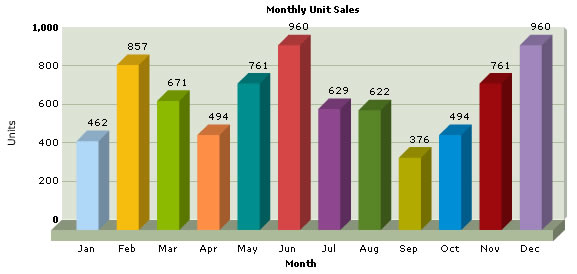
\includegraphics[scale=0.6]{../graph/fusionChartsExemple.jpg}
  \caption{Exemple de graphe en colonne 3D avec FusionCharts Free - \url{http://docs.fusioncharts.com/free/}}
\end{figure}
\end{enumerate}


%-------------------------------------------------------------------%
%------------------------JFreeChart---------------------------------%
%-------------------------------------------------------------------%
\subsection{Images de graphes : JFreeChart}
\subsubsection{Présentation}
JFreeChart est une API Java qui permet de créer des graphes et diagrammes en Java. Elle est open source mais la documentation est payante. Elle se présente sous la forme d'une librairie qui peut être intégrée à l'IDE Eclipse.
\begin{figure}[H]
  \center
  
\includegraphics[scale=0.5]{../graph/JFreeChart.png}
  \caption{JFreeChart - \url{http://www.jfree.org/jfreechart/}}
\end{figure}

JFreeChart permet de tracer différents graphes et ce avec une très bonne qualité d'image. On peut par exemple citer les diagrammes en bar (bar charts), les camemberts (pie charts), les histogrammes, parmis bien d'autres.

Pour utiliser cette librairie, il suffit de la télécharger sur le site suivant : \url{https://sourceforge.net/projects/jfreechart/files/}.
Il faut ensuite extraire l'archive et intégrer le .jar au projet dans Eclipse.

\subsubsection{Mise en place}
Nous allons aborder l'utilisation de JFreeChart avec des JSP. Le principe est que nous allons créer le graphe puis l'enregistrer sous forme d'image. Nous afficherons ensuite l'image dans la page web que l'on souhaite.\\

Il faut donc :
\begin{enumerate}
 \item Créer le graphe dans une JSP et le sauvegarder en variable de session par exemple.
 \item Créer l'image 'map' à partir de ce graphe.
 \item Récupérer l'image dans la servlet et l'enregistrer sous forme de fichier.
 \item Afficher l'image dans la JSP correspondant à la page web dans laquelle on souhaite visualiser le graphe.
\end{enumerate}

Une simplification est d'utiliser Cewolf qui est basé sur JFreeChart et peut être utilisé dans une application web basée sur les JSP et les servlets. En utilisant Cewolf, on n'a plus besoin de stocker l'image car tout se fait de manière dynamique.\\
\begin{figure}[H]
  \center
  
\includegraphics[scale=0.5]{../graph/Cewolf.png}
  \caption{Cewolf - \url{http://cewolf.sourceforge.net/new/index.html}}
\end{figure}

Cewolf est bien documenté est on peut réaliser notre graphique en suivant les étapes suivantes :
\begin{enumerate}
 \item \textbf{Préparer l'application :} ajouter les librairies (.jar) dans le dossier /WEB-INF/lib du projet disponible sur la page \url{https://sourceforge.net/projects/cewolf/files/}.
 \item \textbf{Préparer les données :} créer un objet qui implémente l'interface DatasetProducer (propre à Cewolf). Cela revient à créer une classe qui implémente cette interface. Elle devra implémenter les méthodes \textit{produceDataset()} (pour les données du graphe), \textit{hasExpired} (pour savoir si les données ne sont plus à jour) et \textit{getProducerId()} (identifie le type de DatasetProducer, si deux ont le même ID, ils produisent les même données).
 \item \textbf{Ajouter la servlet Cewolf à l'application :} la classe servlet est déjà fournie avec Cewolf, il suffit de l'ajouter au fichier de configuration web.xml.
 \item \textbf{Définir le graphe dans la JSP :} à l'aide des balises (tags) \textit{<cewolf:chart>}, \textit{<cewolf:data>} et \textit{<cewolf:img>} on intègre l'image à la page JSP dans le bloc HTML. On peut y préciser le titre du graphe, les axes, les dimensions, etc...
\end{enumerate}

La mise en place est assez complexe, mais au final on peut obtenir des graphes sous forme d'image comme les suivants :
\begin{figure}[H]
  \center
  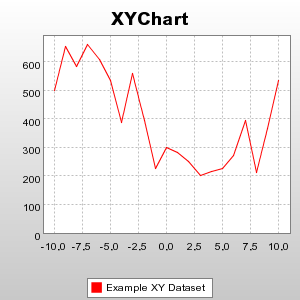
\includegraphics[scale=0.5]{../graph/cewolfEx1.png}
  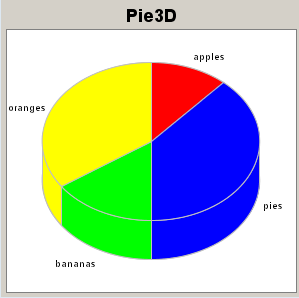
\includegraphics[scale=0.5]{../graph/cewolfEx2.png} 
  \caption{Exemples avec Cewolf - \url{http://cewolf.sourceforge.net/new/index.html}}
\end{figure}

%-------------------------------------------------------------------%
%------------------------GoogleChart--------------------------------%
%-------------------------------------------------------------------%
\subsection{Javascript : API Google Chart}
\subsubsection{Présentation}
L'API Google Chart est un outil qui permet de créer facilement des graphes à partir de données et de l'afficher dans une page web. Les graphes sont intéractifs et peuvent être personnalisé. Il existe de nombreux types de graphes disponibles allant du graphe linéaire à l'histogramme en passant par des organigrammes ou encore des cartes géographiques.\\
\begin{figure}[H]
  \center
  
\includegraphics[scale=0.5]{../graph/googleAPI.png}
  \caption{API Google Chart - \url{https://developers.google.com/chart/}}
\end{figure}

Cette API se met en place en Javascript sans que l'on est besoin de télécharger quoi que ce soit. Il suffit d'avoir une connexion Internet pour afficher les graphes.

\subsubsection{Mise en place}
Pour utiliser les graphes mis à disposition par Google, il faut suivre le schéma suivant et écrire le code dans les balises HTML de la page JSP dans laquelle on souhaite afficher un graphe :
\begin{enumerate}
 \item \textbf{Charger la librairie :} nous n'aurons besoin que de graphes classiques, c'est pourquoi on charge uniquement le package intitulé 'corechart'. Le mot clé 'current' signifie que l'on veut charger la dernière mise à jour officielle et validée par Google Charts. De plus, on suppose que l'on aura une fonction JavaScript plus loin dans le code intitulée 'drawChart'.
\begin{lstlisting}
<script type="text/javascript" src="https://www.gstatic.com/charts/loader.js"></script>
<script type="text/javascript">
    google.charts.load('current', {packages: ['corechart']});
    google.charts.setOnLoadCallback(drawChart);
</script>
\end{lstlisting}
 \item \textbf{Préparer les données :} l'API requiert d'avoir les données sous forme d'une 'DataTable' qui est une classe Javascript définie dans la librairie Google Visualization chargée à l'étape précédente. Une DataTable est un tableau à deux dimensions donc les colonnes sont les types de données et les lignes les données elle-mêmes. Il existe différentes manières de créer une DataTable mais il est important qu'elle soit toujours adaptée au type de graphe qui sera créé (par exemple pour un camembert il faudra toujours deux colonnes). Il est possible d'instancier la DataTable de manière statique ou dynamique. Remarque : tous les morceaux de code qui suivent devront être placés dans une fonction Javascript \textit{drawChart} comme précisé précédemment.
\begin{lstlisting}
// Creation de la DataTable avec deux colonnes et trois lignes :
var data = new google.visualization.DataTable();
data.addColumn('string', 'Actifs');
data.addColumn('number', 'Quantite');
data.addRows([
    ['Obligation', 76.7],
    ['Action', 23.3]
]);
\end{lstlisting}
 \item \textbf{Personnaliser le graphe :} il est possible de spécifier certaines options à l'API comme les couleurs de chaque partie du graphique, la police, la taille, le titre, les légendes, etc...
\begin{lstlisting} 
var options = {
    backgroundColor: '#d2d2d2',
    title: 'Repartition du portefeuille selon la somme investie',
    is3D: true,
    width:400,
    height:300
};
\end{lstlisting}
 \item \textbf{Dessiner le graphe :} c'est ici que l'on va préciser à l'API quel type de graphe on souhaite dessiner, avec quelles données et options. On affectera alors un ID au graphique qui servira dans la dernière étape. Remarque : après ces deux lignes, la fonction \textit{drawChart} est finie.
\begin{lstlisting}
var chart = new google.visualization.PieChart(document.getElementById('camembert'));
chart.draw(data, options);
\end{lstlisting} 
 \item \textbf{Afficher le graphe :} il ne reste plus qu'à choisir l'emplacement du graphe dans la page web et à insérer la ligne suivante au bon endroit dans le HTML. L'ID devra être exactement le même que celui donné dans l'étape précédente.
\begin{lstlisting}
<div id="camembert"></div>
\end{lstlisting}  
 
 On est censé voir s'afficher ceci :
\begin{figure}[H]
  \center
  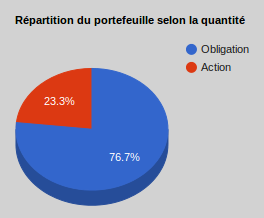
\includegraphics[scale=0.6]{../graph/camembertAPI.png}
  \caption{Exemple diagramme Camembert (Pie Chart)}
\end{figure}
\end{enumerate}


%-------------------------------------------------------------------%
%------------------------notrechoix---------------------------------%
%-------------------------------------------------------------------%
\subsection{Notre choix}
Maintenant que nous avons étudié les différentes options qui s'offrent à nous, nous pouvons discuter la meilleure solution à adopter. Tout d'abord, il apparait clairement que la méthode utilisant Flash est désuette bien qu'elle doit fonctionner sans problème. Nous n'avons donc même pas essayé de l'implémenter.\\

En ce qui concerne la librairie JFreeChart, c'est la première à laquelle nous avons pensé et que nous avons essayé de mettre en oeuvre. Après avoir rencontré quelques difficultés dans la mise en place de cette solution, nous avons réfléchis à une autre solution. En effet, nous perdions trop de temps à essayer d'utiliser JFreeChart et Cewolf, sans parler du fait que cela nécessitait l'ajout de librairie à notre projet.\\

Ainsi, nous nous sommes finalement retrouvé à utiliser l'API Google Chart qui, pour le coup, est très simple à utiliser car elle est gérée uniquement dans les JSP. De plus, nous trouvons que les graphes mis à disposition sont satisfaisants et que l'intéractivité avec les diagrammes peut avoir des avantages lors de l'analyse des graphes.\\

Nous avons néanmoins rencontré quelques difficultés avec les DataTable lorsque nous avons voulu les définir de manière dynamique, mais nous avons finalement réussi et ce notamment grâce à la librairie JSTL que nous avons défini auparavant.